\chapter{Diagnostic Tool}
The MOEA Framework provides a graphical interface to quickly run and analyze MOEAs on a number of test problems.  This chapter describes this diagnostic tool in detail.

\section{Running the Diagnostic Tool}
The diagnostic tool is launched in a number of ways, depending on which version of the MOEA Framework you downloaded.  Follow the instructions below for your version to launch the diagnostic tool.

\paragraph{Compiled Binaries}
Run \file{launch-diagnostic-tool.bat} on Windows.  You can manually run the diagnostic tool with the following command:

\begin{lstlisting}[language=Plaintext]
java -Djava.ext.dirs=lib
		org.moeaframework.analysis.diagnostics.LaunchDiagnosticTool
\end{lstlisting}

\paragraph{All-in-One Executable}
Double-click the downloaded JAR file.  If this fails, you can also manually launch the tool with with the following command:

\begin{lstlisting}[language=Plaintext]
java -jar MOEAFramework-%VERSION%-Executable.jar
\end{lstlisting}

\paragraph{Source Code}
Inside Eclipse, navigate to the src $\rightarrow$ org $\rightarrow$ moeaframework $\rightarrow$ analysis $\rightarrow$ diagnostic package in the Package Explorer window.  Right-click the file \texttt{LaunchDiagnosticTool.java} and select the Run as $\rightarrow$ Java Application option in the popup menu.

\section{Layout of the GUI}

\figref{fig:diagnosticToolAnnotated} provides a screenshot of the diagnostic tool window.  This window is composed of the following sections:

\begin{figure}
  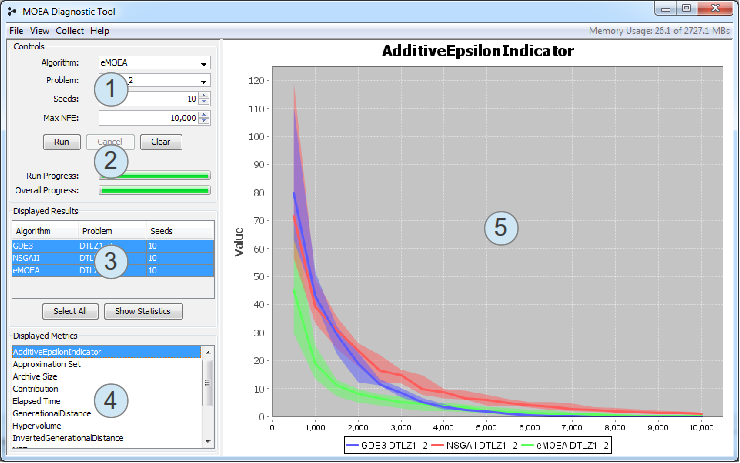
\includegraphics[width=\linewidth]{diagnosticToolAnnotated.png}
  \caption{The main window of the diagnostic tool.}
  \label{fig:diagnosticToolAnnotated}
\end{figure}

\begin{enumerate}
  \item The configuration panel.  This panel lets you select the algorithm, problem, number of repetitions (seeds), and maximum number of evaluations (NFE).
  \item The execution panel.  Clicking run will execute the algorithm as configured in the configuration panel.  Two progress bars display the individual run progress and the total progress for all seeds.  Any in-progress runs can be canceled.
  \item The displayed results table.  This table displays the completed runs.  The entries which are selected/highlighted are displayed in the charts.  You can click an individual line to show the data for just that entry, click while holding the Alt key to select multiple entries, or click the Select All button to select all entries.
  \item The displayed metrics table.  Similar to the displayed results table, the selected metrics are displayed in the charts.  You can select one metric or multiple metrics by holding the Alt key while clicking.
  \item The actual charts.  A chart will be generated for each selected metric.  Thus, if two metrics are selected, then two charts will be displayed side-by-side.  See \figref{fig:diagnosticToolMultiselect} for an example.
\end{enumerate}

\begin{figure}
  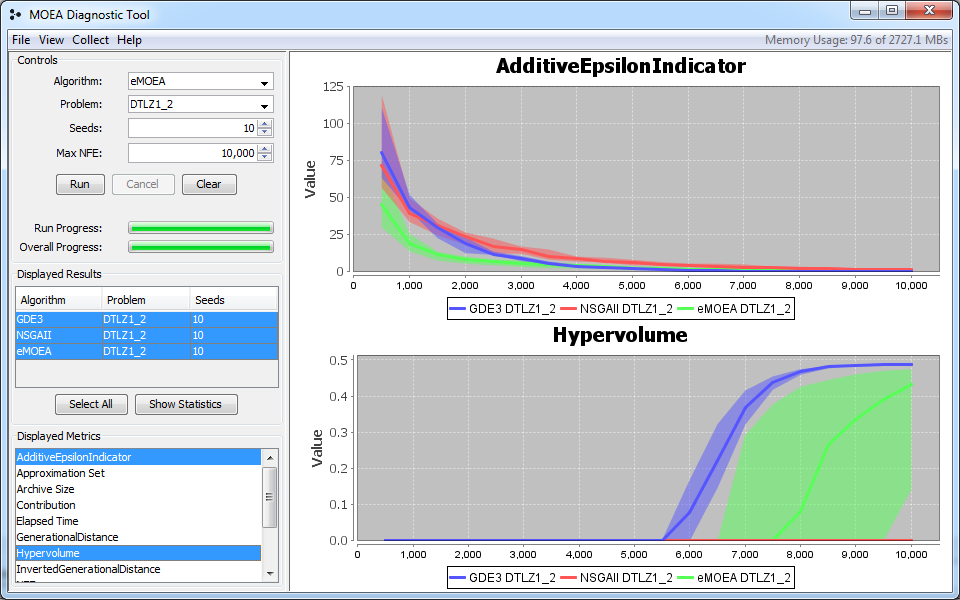
\includegraphics[width=\linewidth]{diagnosticToolMultiselect.png}
  \caption{Screenshot of the diagnostic tool displaying two side-by-side metrics.  You can select as many metrics to display by holding down the Alt key and clicking a row in the displayed metrics table.}
  \label{fig:diagnosticToolMultiselect}
\end{figure}

\begin{tip}
  Some algorithms do not provide certain metrics.  When selecting a specific metric, only those algorithms that provide that metric will be displayed in the chart.
\end{tip}

\section{Quantile Plots vs Individual Traces}
By default, the chart displayed by the diagnostic tool show the statistical 25\%, 50\% and 75\% quantiles.  The 50\% quantile is the thick colored line, and the 25\% and 75\% quantiles are depicted by the colored area.  This quantile view allows you to quickly distinguish the performance between multiple algorithms, particularly when there is significant overlap between two or more algorithms.

You can also view the raw, individual traces by selecting 'Show Individual Traces' in the View menu.  Each colored line represents one seed.  \figref{fig:diagnosticToolTraces} provides an example of plots showing individual traces.  You can always switch back to the quantile view using the View menu.

\begin{figure}
  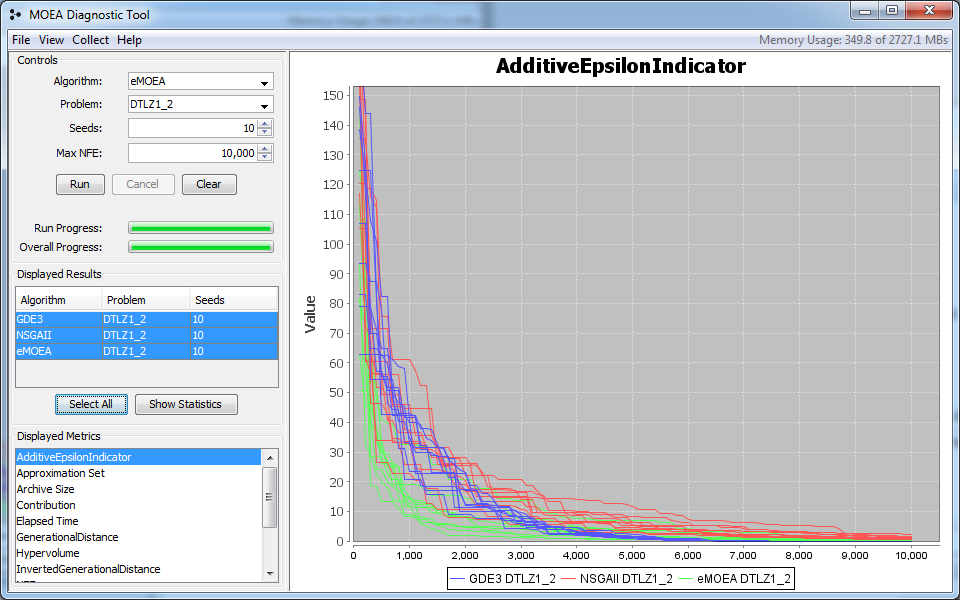
\includegraphics[width=\linewidth]{diagnosticToolTraces.png}
  \caption{Screenshot of the diagnostic tool displaying the individual traces rather than the quantile view.  The individual traces provide access to the raw data, but the quantile view is often easier to interpret.}
  \label{fig:diagnosticToolTraces}
\end{figure}

\section{Viewing Approximation Set Dynamics}
Another powerful feature of the diagnostic tool is the visualization of approximation set dynamics.  The approximation set dynamics show how the algorithm's result (its approximation set) evolved throughout the run.  To view the approximation set dynamics, right-click on one of the rows in the displayed results table.  A menu will appear with the option to show the approximation set.  A window similar to \figref{fig:approximationSetViewerAnnotated} will appear.

\begin{important}
  This menu will disappear if you disable collecting the approximation set using the Collect menu.  Storing the approximation set data tends to be memory intensive, and it is sometimes useful to disable collecting the approximation sets if they are not needed.
\end{important}

\begin{figure}
  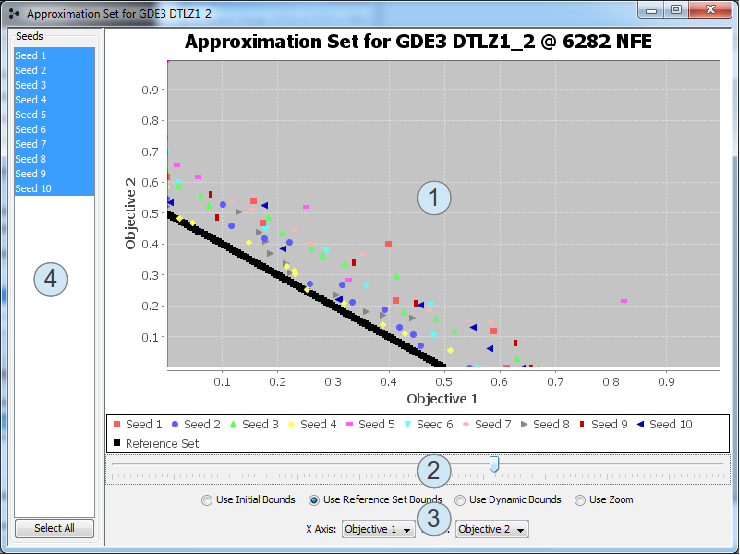
\includegraphics[width=\linewidth]{approximationSetViewerAnnotated.png}
  \caption{Screenshot of the approximation set viewer.  This allows you to view the approximation set at any point in the algorithm's execution.}
  \label{fig:approximationSetViewerAnnotated}
\end{figure}

This window displays the following items:

\begin{enumerate}
  \item The approximation set plot.  This plot can only show two dimensions.  If available, the reference set for the problem will be shown as black points.  All other points are the solutions produced by the algorithm.  Different seeds are displayed in different colors.
  \item The evolution slider.  Dragging the slider to the left or right will show the approximation set from earlier or later in the evolution.
  \item The display controls.  These controls let you adjust how the data is displayed.  Each of the radio buttons switches between different scaling options.  The most common option is 'Use Reference Set Bounds', which scales the plot so that the reference set fills most of the displayed region.
  \item The displayed seeds table.  By default, the approximation sets for all seeds are displayed and are distinguished by color.  You can also downselect to display one or a selected group of seeds by selecting entries in this table.  Multiple entries can be selected by holding the Alt key while clicking.
\end{enumerate}

\begin{tip}
  You can manually zoom to any portion in these plots (both in the approximation set viewer and the plots in the main diagnostic tool window) by positioning the cursor at the top-left corner of the zoom region, pressing and holding down the left-mouse button, dragging the cursor to the bottom-right corner of the zoom region, and releasing the left-mouse button.  You can reset the zoom by pressing and holding the left-mouse button, dragging the cursor to the top-left portion of the plot, and releasing the left-mouse button.
\end{tip}

\section{Statistical Results}
The diagnostic tool also allows you to exercise the statistical testing tools provided by the MOEA Framework with the click of a button.  If you have two or more entries selected in the displayed results table, the 'Show Statistics' button will become enabled.  \figref{fig:statisticalResultsViewer} shows the example output from clicking this button.  The data is formatted as YAML.  YAML uses indentation to indicate the relationship among entries.  For example, observe that the first line is not indented and says 'GDE3:'.  All entries shown below that are indented.  Thus, the second line, which is 'Hypervolume:', indicates that this is the hypervolume for the GDE3 algorithm.  The third line says 'Aggregate: 0.4894457739242269', and indicates that the aggregate hypervolume produced by GDE3 was $0.489$.

\begin{figure}
  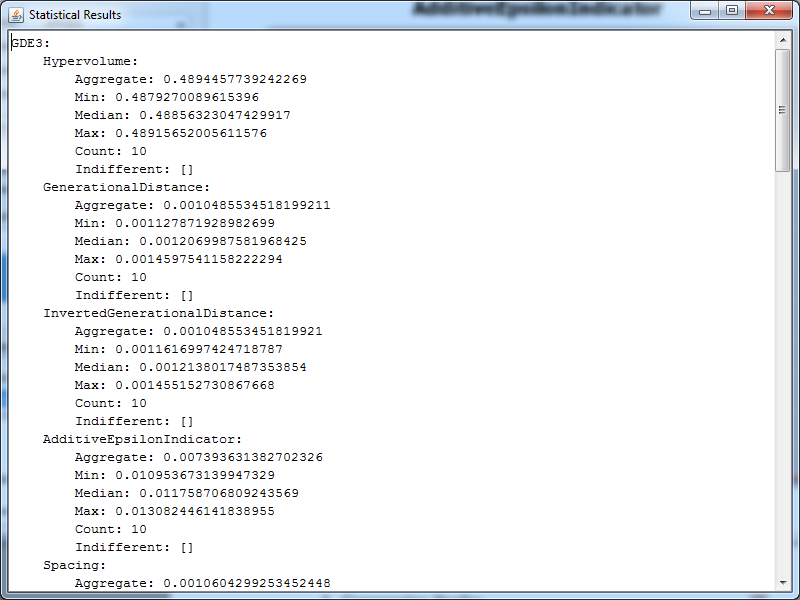
\includegraphics[width=\linewidth]{statisticalResultsViewer.png}
  \caption{Screenshot of the statistics output by the diagnostic tool.}
  \label{fig:statisticalResultsViewer}
\end{figure}

Displayed for each metric are the min, median and max values for the specific metric.  It is important to note that these values are calculated from the end-of-run result.  No intermediate results are used in the statistical tests.  The aggregate value is the metric value resulting when the result from all seeds is combined into one.  The count is the number of seeds.  

The indifferent entries are of particular importance and will be explained in detail.  When comparing two data sets using statistical tools, it is not sufficient to simply compare their average or median values.  This is because such results can be skewed by randomness.  For example, suppose we are calculating the median values of ten seeds.  If one algorithm gets ``lucky'', and happens to use more above-average seeds, the estimated median will be skewed.  Therefore, it is necessary to check the statistical significance of results.  This is exactly what the indifferent entries are displaying.  To determine statistical significance, the MOEA Framework uses the Kruskal-Wallis and Mann-Whitney U tests with 95\% confidence intervals.  If an algorithm's median value for a metric is statistically different from another algorithm, the indifferent entry will contain an empty list (e.g., 'Indifferent: []').  However, if its results are not statistically different, then the indifferent entry will list the algorithms it is statistically inidifferent (e.g., 'Indifferent: [NSGAII]').  This list may contain more than one algorithm if multiple algorithms are indifferent.

\begin{important}
  The show statistics button also requires each of the selected entries to use the same problem.  The button will remain disabled unless this condition is satisfied.
\end{important}

\section{Advanced Use}
This last section details some more advanced use of the diagnostic tool.

\subsection{Improving Performance and Memory Efficiency}
By default, the diagnostic tool collects and displays all available data.  If you know ahead of time that certain pieces of data are not needed for your experiments, you can often increase the performance and memory efficiency of the program by disabling unneeded data.  You can enable or disable the collection of data by checking or unchecking the appropriate item in the Collect menu.